\documentclass[../tesis_main.text]{subfiles}


\chapter{Implementación usando la plataforma ROS}
	\addtocounter{page}{-1}
	
	En este capítulo se describe la plataforma ROS (Robot Operative System), su estructura, los elementos principales que lo componen y sus formas de interconección. Se aborda, además, la metodología de integración de los algoritmos desarrollados en este trabajo.\\ 

	\section{Ros}
	ROS es un meta-sistema operativo de software libre para robótica que ofrece las utilidades que se esperarían en cualquier sistema operativo: abstracción de hardware, control de dispositivos de bajo nivel, implementación de funcionalidades comunes, intercambio de mensajes entre procesos y mantenimiento de paquetes. Su objetivo principal es dar soporte a la reutilización de código en la investigación y desarrollo de robótica \cite{quigley2009ros}.\\

	Una de las principales ventajas que ofrece es la de comunicar distintos procesos dependientes o independientes entre sí de manera muy sencilla. El funcionamiento de un robot se piensa de manera modular, donde cada módulo realiza una tarea específica y ROS se encarga del transporte de la información entre ellos. Además, su creciente comunidad aporta mucho al desarrollo de nuevo software que otros usuarios pueden utilizar de acuerdo a sus necesidades.\\

	\subsection{Nodos}
	Nodo es el nombre que reciben ROS los pequeños módulos que conforman la red de trabajo; se encargan de realizar una tarea en particular. Por ejemplo, un nodo mueve los motores, otro nodo es responsable de la interfaz con el usuario, otro planea las trayectorias, mientras que un último nodo controla los sensores. La comunicación entre nodos se realiza por medio de mensajes usando tópicos o servicios.\\

	\subsection{Paquetes}
	El software en ROS se organiza por medio de paquetes. Un paquete puede entenderse como una carpeta con estructura definida y puede contener el código de un nodo, la definición de mensajes, archivos de configuración, software ajeno a ROS, etc. Se pretende que un paquete ofrezca una utilidad por sí mismo, pero no debe ser tan complejo como para ser difícil de entender por otros usuarios. Cuando se comparten desarrollos en la comunidad de ROS, los paquetes son la unidad más pequeña de construir y publicar. Es decir, si se crea un nodo con una funcionalidad única y éste se quiere compartir con el mundo, lo que se debe compartir en realidad es el paquete que contiene al nodo.\\

	\subsection{Tópicos}
	Uno de los patrones para comunicar nodos entre sí es por medio de tópicos. Un nodo publica cierto tipo de información en un tópico específico y todos los nodos que requieran de esa información deberán suscribirse a ese tópico para obtenerla. En cuanto los datos sean publicados, los nodos suscritos la recibirán. Los tópicos son un patrón no-bloqueante que presenta una distribución 1:n.\\

	\subsection{Servicios}
	El otro patrón para comunicar nodos son los servicios, que utilizan un sistema petición-respuesta. Si algún proceso o cálculo se requiere hacer sólo en ciertas situaciones es conveniente programarlo como un servicio. Si un nodo requiere utilizar un servicio, manda un mensaje de petición con la información necesaria al nodo que ofrece dicho servicio, el procesamiento se lleva a cabo y se regresa al nodo solicitante un mensaje de respuesta con el resultado del servicio. Al igual que los tópicos, cada servicio tiene el tipo de mensaje específico con el que se comunicará; hay un tipo de mensaje para las peticiones y otro para las respuestas.\\	

	\begin{figure}[H]
		% \hspace*{-0.15in}
		\begin{center}
		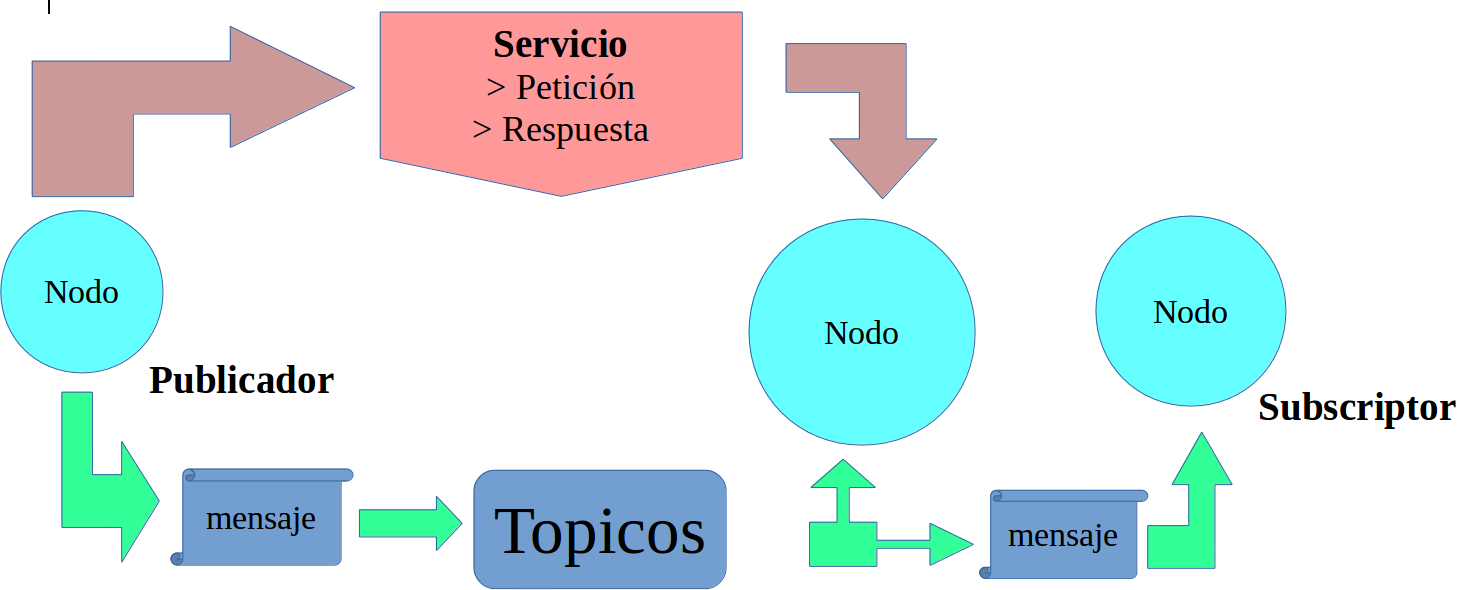
\includegraphics[scale=0.28]{ros/topics_services_ros.png}	
		\caption{Esquemas de comunicación Tópicos y Servicios.}
		\end{center}
	\end{figure}





	%%%%
	%%%%   Desarrollo de pruebas
	%%%%
	\section{Máquinas de estados}

	Se denomina máquina de estados a un modelo de comportamiento de un sistema con entradas y salidas, en donde las salidas dependen no sólo de las señales de entradas actuales sino también de las anteriores.\\

	Las máquinas de estados se definen como un conjunto de estados que sirve de intermediario en esta relación de entradas y salidas, haciendo que el historial de señales de entrada determine, para cada instante, un estado para la máquina, de forma tal que la salida depende únicamente del estado y las entradas actuales.\\

	En este sentido, como parte de este trabajo, se plantean las máquinas de estados como la metodología de solución ante ciertos problemas como lo son: \textit{describir el proceso de la toma de objetos, describir el proceso de llevar el brazo hasta el punto óptimo de sujeción, describir el proceso de evaluación de la función de costo para el brazo manipulador del robot Justina, entre otras.}\\

	\begin{figure}[H]
		% \hspace*{-0.15in}
		\begin{center}
		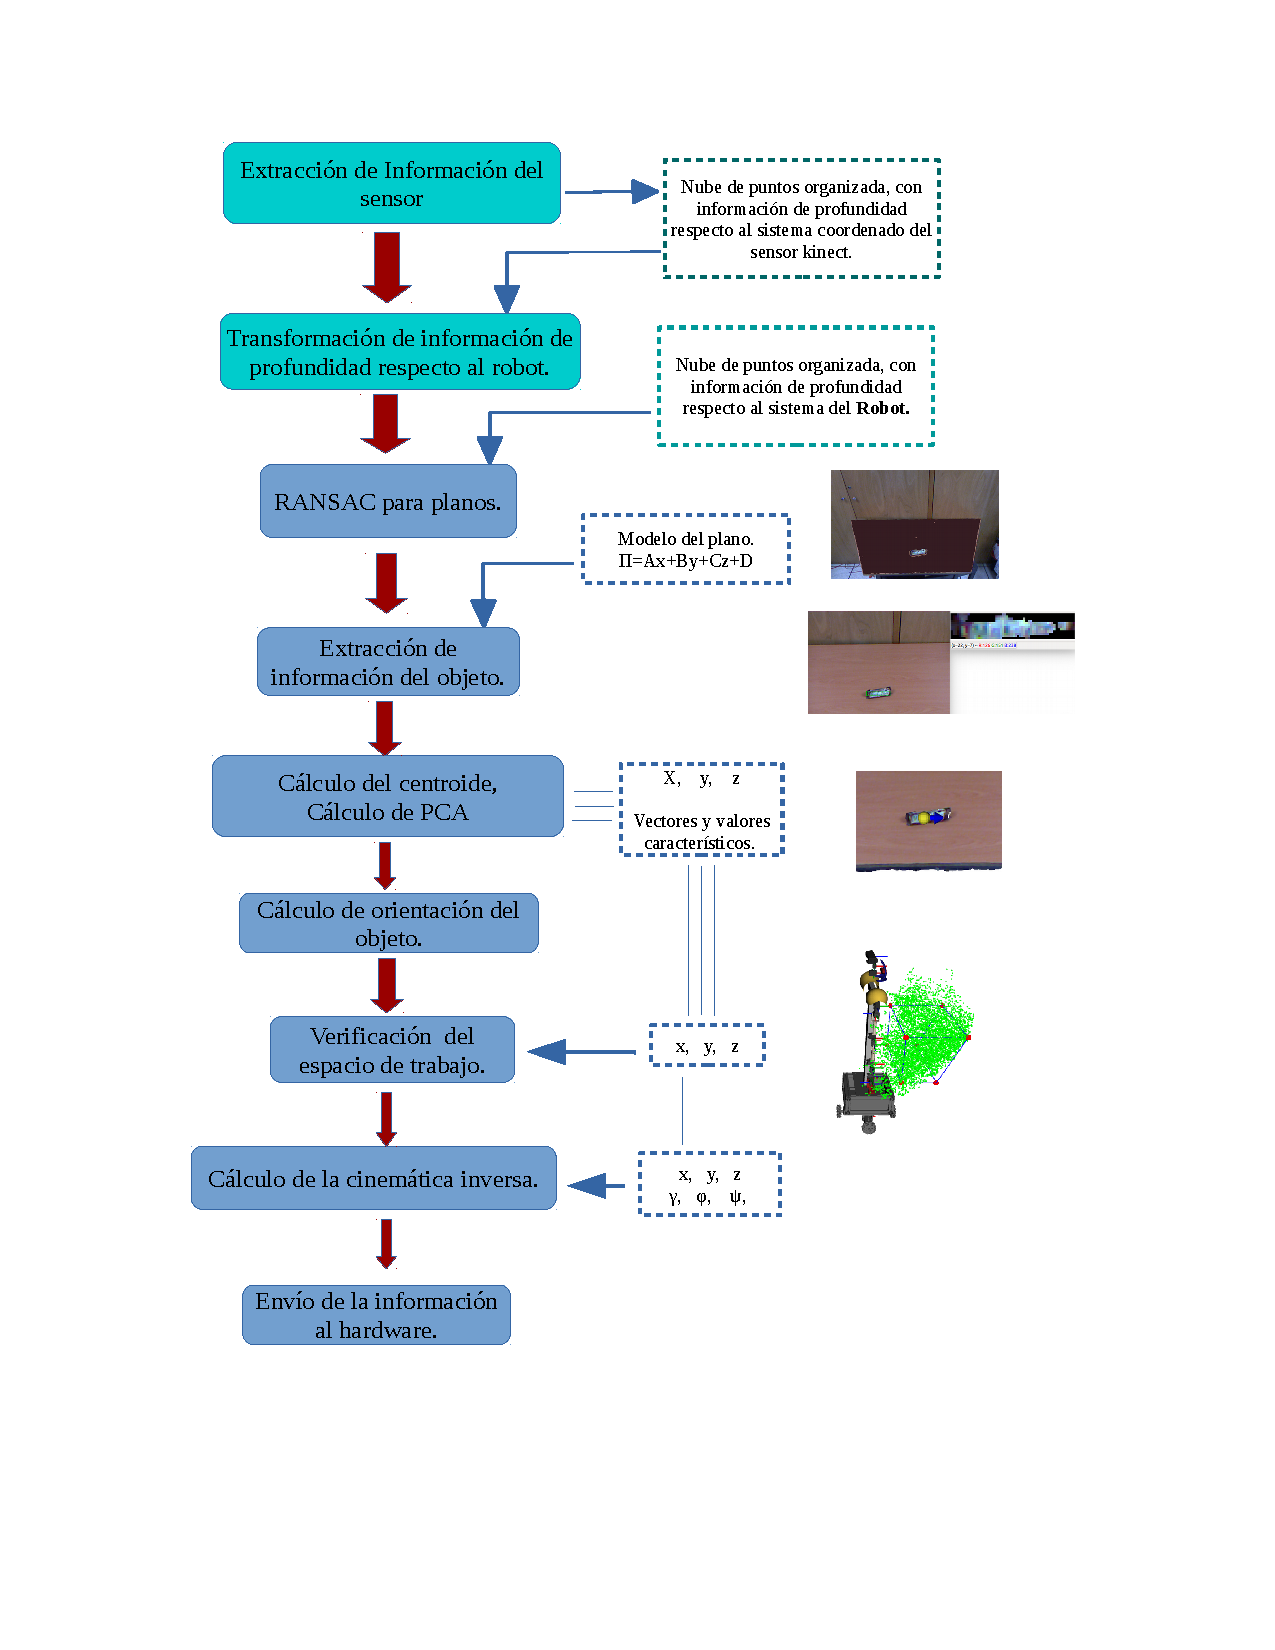
\includegraphics[scale=0.70]{ros/bloquesSistema.pdf}	
		\caption{Diagrama de bloques del sistema de manipulación.}
		\end{center}
	\end{figure}


	\subsection{Descripción de pruebas de toma de objetos.}

	La toma de objetos es la parte crucial de este trabajo, la importancia de este evento radica en que se incluye la totalidad de tareas desarrolladas en este trabajo para realizar una prueba de mayor complejidad. A grandes rasgos, la prueba de la toma de objetos se compone de subtareas, algunas de las cuales se describen a continuación.\\

	La primer subtarea es la segmentación del objeto y el cálculo del respectivo centroide del objeto en cuestión (Ver Sección [3]). Como entrada de la tarea se tiene una nube de puntos obtenida por la cámara RGB-D Kinect y lo esperado a la salida es una posición \textit{x, y, z} en el espació así como la orientación del objeto \textit{roll, pith, yaw}. Partiendo con la nube de puntos como entrada al sistema, es la segmentación de un plano (en caso de existir), posteriormente se eliminan los puntos pertenecientes al plano y por debajo de este, se eliminan los puntos más alejados 0,5[m] en el eje x respecto al robot. Se parte de las siguientes premisas: que el conjunto de puntos restante corresponde al conjunto de puntos que conforman al objeto, que solo se encuentra un objeto en la mesa en cada evento de toma de objetos. Con tal información, podemos proceder a calcular el centroide del objeto así como el respectivo ángulo del mismo.\\

	\begin{figure}[H]
	%\hspace*{-0.5in}
	\centering
	\begin{subfigure}[t]{.55\textwidth}
		\centering
		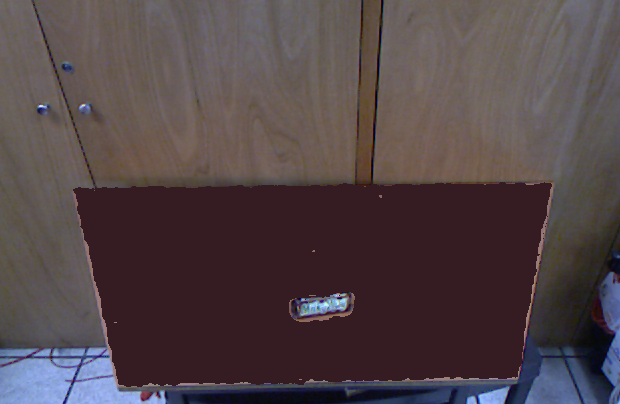
\includegraphics[scale=0.25]{objs/plane_model.png}
		\caption{Imagen de segmentación de los puntos \\ pertenecientes al plano.}
	\end{subfigure}%
	\begin{subfigure}[t]{.55\textwidth}
		\centering
		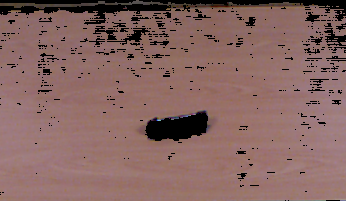
\includegraphics[scale=0.45]{objs/plane_points.png}
		\caption{Segmentación de plano con extracción \\ de los objetos sobre este.}
	\end{subfigure}

	\hspace*{-0.5in}
	\begin{subfigure}[t]{.55\textwidth}
		\centering
		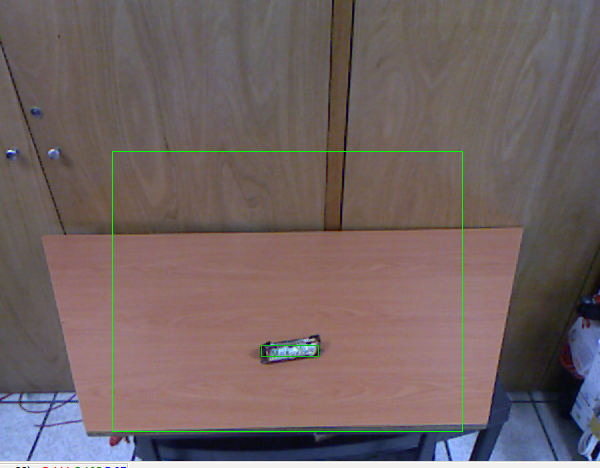
\includegraphics[scale=0.25]{objs/object_boundingBox.png}
		\caption{Boundig box de la región de interes.}
	\end{subfigure}%
	\begin{subfigure}[t]{.55\textwidth}
		\centering
		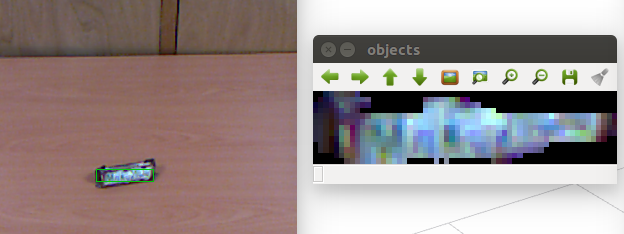
\includegraphics[scale=0.45]{objs/object_points.png}
		\caption{Bounding box de los puntos pertenecientes al objeto.}
	\end{subfigure}
	\caption{Esquemas del proceso de segmentación del objeto.}
	\label{fig:desciption_arms1}
	\end{figure}


	Para realizar el cálculo del centroide del objeto en cuestión se utiliza la media en cada uno de los correspondientes ejes, el cálculo es prácticamente directo, no así el cálculo de los ángulos representativos de la orientación del objeto. Para ello se calculó en un principio, los componentes principales del conjunto formado por los puntos del objeto, con la información de los eigenvectores de la matriz de covarianzas podemos obtener la dirección en la cuál ocurre la mayor distribución de los puntos, y por tanto podemos obtener los cosenos directores de cada uno de los respectivos eigenvectores obteniendo así los ángulos de rotación \textit{roll, pitch, yaw}.\\


	Una vez conociendo esta información es posible avanzar a la etapa de manipulación para la cual es necesario conocer la información del objeto en el espacio \textit{x, y, z} y con ayuda del proceso anteriormente descrito podemos obtener los ángulos requeridos para el efector final del manipulador. En esta etapa como parte de los resultados del análisis comparativo entre las soluciones encontradas mediante la paquetería \textit{MoveIt!} y el método geométrico, se optó por utilizar el método geométrico ya implementado en el robot de servicio Justina.\\



	\begin{figure}[H]
		\begin{center}
		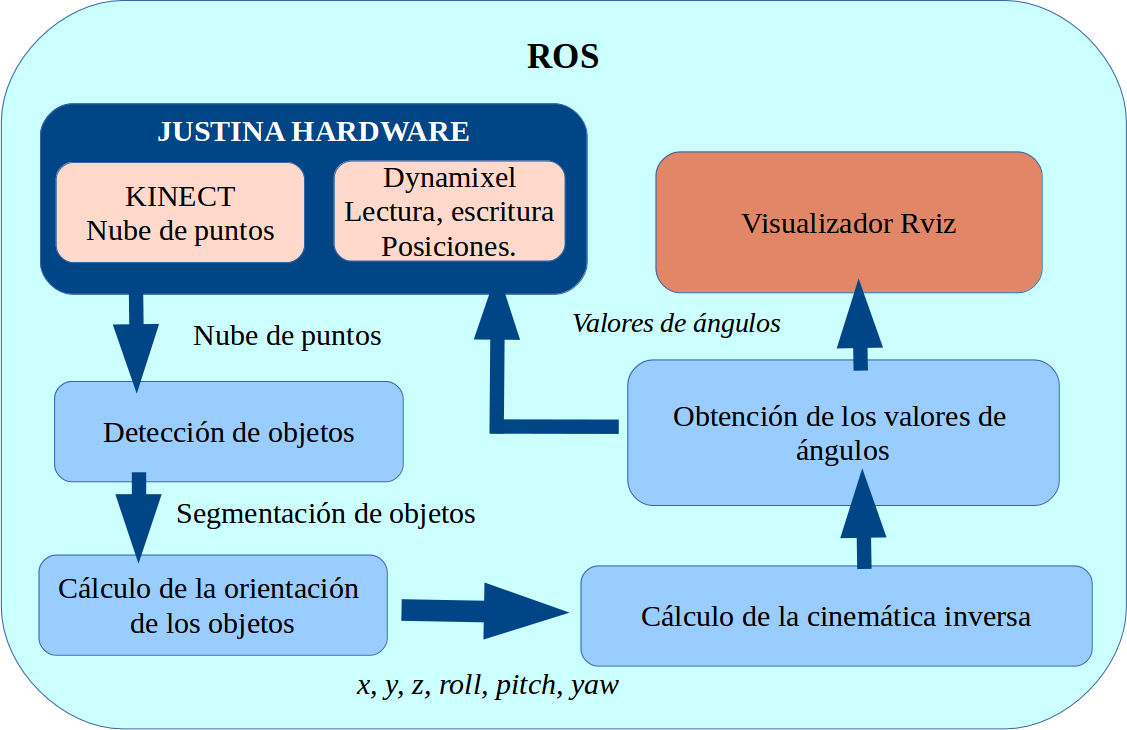
\includegraphics[scale=0.20]{ros/tarea_manipulacion2.png}	
		\caption{Diagrama de bloques del proceso toma de objetos.}
		\end{center}
	\end{figure}



	Con el resultado del cálculo de la cinemática inversa, se obtienen los ángulos requeridos para cada uno de los actuadores para que el efector final llegue al punto en el espacio deseado. Para ello se utiliza un \textit{tópico} implementado en ROS, que comunica los ángulos deseados del manipulador con un nodo encargado de operar el hardware, en este caso, los motores Dynamixel.\\ 


	\subsection{Pruebas de toma de objetos estado actual.}

	En lo que respecta al proceso de la toma de objetos actual, en el robot de servicio Justina, unicamente se utiliza la información de posición del objeto sin considerar la información de orientación. Este proceso es susceptible a fallas cuando se trata de objetos de grandes dimensiones, entiéndase objetos con dimensiones mayores a la longitud total del efector final del manipulador en su mayor apertura. Por otro lado, puede presentar fallas con objetos de alturas reducidas, estos son objetos con alturas menores a la mitad de la longitud \textit{d} del manipulador pues ello indica una posible colisión con la superficie que soporta dicho objeto.\\

	\begin{figure}[H]
	\hspace*{-0.5in}
	\centering
	\begin{subfigure}[t]{.55\textwidth}
		\centering
		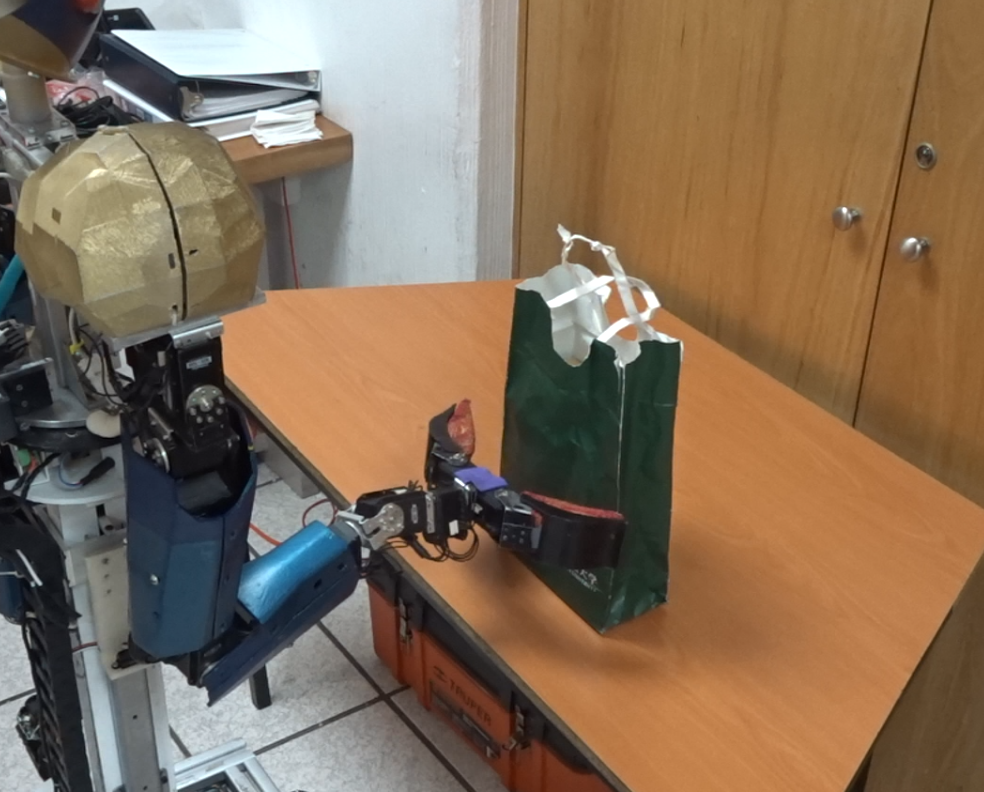
\includegraphics[scale=0.18]{objs_real/bag_unsuccess.png}
		\caption{Sin considerar información de orientación.}
	\end{subfigure}%
	\begin{subfigure}[t]{.55\textwidth}
		\centering
		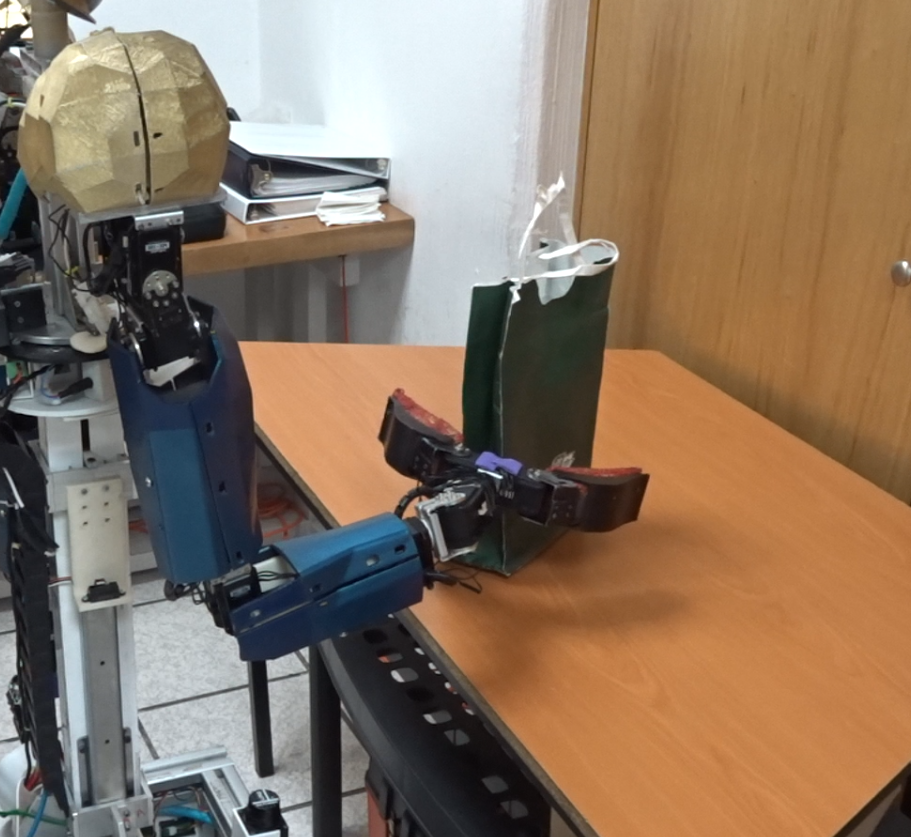
\includegraphics[scale=0.18]{objs_real/bag_success.png}
		\caption{Tomando en cuenta la información de orientación.}
	\end{subfigure}
	\caption{Fotografía de la tarea de manipulación para una bolsa de papel.}
	\label{fig:grasp_task}
	\end{figure}	

	
	\subsection{Pruebas de toma de objetos con información de orientación y dimensiones del objeto.}

	Como parte de los desarrollos obtenidos de este trabajo, se adiciona la información de la orientación de los objetos, con la cual se puso a prueba si la adición de esta información mejora significativamente la tarea de toma de objetos en el robot de servicio Justina.\\

	Para ello, una vez realizada la segmentación del objeto en cuestión se procede a calcular el centroide del objeto, posteriormente se calcula la matriz de covarianzas de y se obtienen los vectores y valores característicos de la matriz, con lo cual se obtienen los ejes que representan una aproximación a la orientación del objeto.\\ 

	\IncMargin{1em}
	\begin{algorithm}[H]
		\SetKwData{Left}{left}\SetKwData{This}{this}\SetKwData{Up}{up}
		\SetKwFunction{Union}{Union}\SetKwFunction{FindCompress}{FindCompress}
		\SetKwInOut{Input}{input}\SetKwInOut{Output}{output}
		
		\Input{Vectores principales del objeto}
		\Output{Ángulos del efector final $roll (\phi), pitch(\theta), yaw(\psi) $}
		\BlankLine
	
		$Inicializaci\acute{o}n$ de $variables$\;
		$\phi   = 0$\;
		$\theta = 0$\;
		$\psi   = 0$\;
		\BlankLine
		\BlankLine

		\SetAlgoLined
		\SetKwProg{Def}{def}{:}{} 
		\Def{ordenamiento vectores($\vec{v_1}, \vec{v_2},\vec{v_3}$)}
		{
			\textbf{return} $ list(\vec{v}_{mayor}, \vec{v}_{medio},\vec{v}_{menor}) $\;
		}
		\BlankLine
		\BlankLine
		\BlankLine

		\SetAlgoLined
		\SetKwProg{Def}{def}{:}{} 
		\Def{etiquetado($\vec{v}$)}
		{
			\textbf{return} $\vec{v} \leftarrow x  \|  y  \|  z $\;
		}
		\BlankLine
		\BlankLine
		\BlankLine


		\SetAlgoLined
		\SetKwProg{Def}{def}{:}{} 
		\Def{main($\vec{v_1}, \vec{v_2},\vec{v_3}$)}
		{
			$\vec{v} \leftarrow $ variable local\;
			$\vec{v}_{mayor}, \vec{v}_{medio},\vec{v}_{menor} \leftarrow $ ordenamientoVectores($\vec{v_1}, \vec{v_2},\vec{v_3}$)\;
			etiquetado($\vec{v}$)\;
			\BlankLine

			\eIf{$\vec{v}_{mayor} == "z"$}
			{
				roll  $\phi =$ 0\;
				pitch $\theta =$ -90\;
				yaw   $\psi = \arctan{ \dfrac{\vec{v}_{menor}.y }{ \vec{v}_{menor}.x} }$\;
			}
			{
				roll  $\phi = \arctan{ \dfrac{\vec{v}_{menor}.y }{ \vec{v}_{menor}.x} }$\;
				pitch $\theta =$ 0\;
				yaw   $\psi =  $ 0\;
		 	}

			\textbf{return} $\phi, \theta, \psi$\;
		}

		\BlankLine
		\BlankLine
		\BlankLine

		\caption{Cálculo de ángulos del efector final de un brazo manipulador con muñeca esférica}
		\label{Alg:angles}
	\end{algorithm}\DecMargin{1em}


	Con fines de obtener el conjunto de ángulos en los cuales debe posicionarse el efector final del manipulador fue preciso realizar dos ordenamientos. El primer ordenamiento se realizó considerando la magnitud de los vectores característicos de la matriz de covarianzas. Posteriormente para cada uno de esos vectores se etiquetó en cuál de los ejes coordenados del sistema de la base del robot sus proyecciones eran mayores. El algoritmo \ref{Alg:angles} menciona los pasos que componen esta tarea.\\

	


	De esta manera la abstracción de la información que tenemos se basa en que sabemos cual es el mayor eje, su magnitud y la dirección a la cual apunta. Por lo tanto, realizamos el siguiente criterio para determinar los ángulos de rotación del efector final.\\


	\begin{figure}[H]
	\hspace*{-0.5in}
	\centering
	\begin{subfigure}[t]{.55\textwidth}
		\centering
		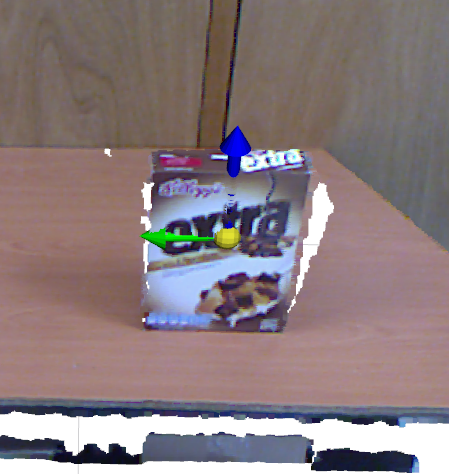
\includegraphics[scale=0.35]{objs/principalAxis_cereal.png}	
		\caption{Caja de cereal}
	\end{subfigure}%
	\begin{subfigure}[t]{.55\textwidth}
		\centering
		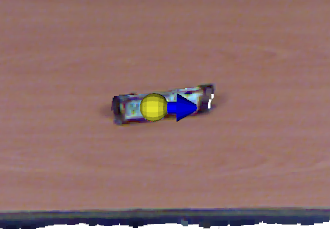
\includegraphics[scale=0.45]{objs/principalAxis_chocolate.png}
		\caption{Barra de chocolate}
	\end{subfigure}

	\hspace*{-0.5in}
	\begin{subfigure}[t]{.55\textwidth}
		\centering
		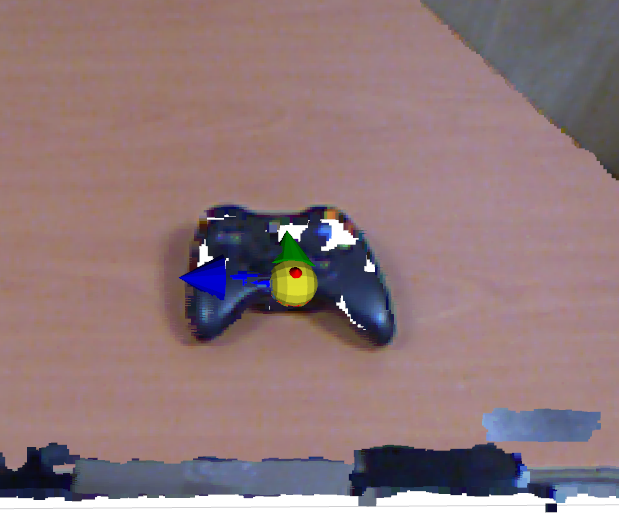
\includegraphics[scale=0.35]{objs/principalAxis_joystick.png}
		\caption{Control de videojuegos}
	\end{subfigure}%
	\begin{subfigure}[t]{.55\textwidth}
		\centering
		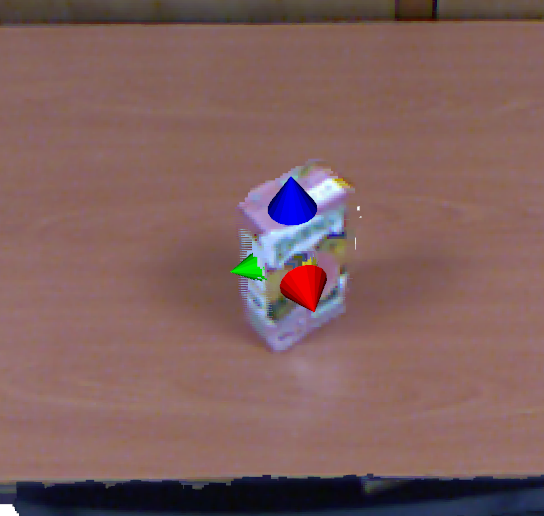
\includegraphics[scale=0.35]{objs/principalAxis_juice2.png}
		\caption{Caja de jugo}
	\end{subfigure}
	\caption{Imagen de cálculo de la orientación con PCA. En azul, el eje con mayor magnitud, que representa el eje en el cual existe una mayor distribución de puntos (eje con mayor varianza de datos).}
	\label{fig:principalVector}
	\end{figure}



	%%%
	%%%	Descripción general del software Justina
	%%%
	\section{El robot de servicio Justina}

	Justina es un robot de servicio desarrollado en el laboratorio de Biorobótica de la Facultad de Ingeniería de la Universidad Nacional Autónoma de México. Dentro del conjunto de tareas que debe desempeñar el robot Justina se encuentran la detección y el reconocimiento de rostros, la detección y el reconocimiento de objetos, la manipulación de objetos, la navegación en un ambiente cerrado similar al de un hogar u oficina, todo esto de manera autónoma.\\

	Para realizar tales tareas el robot de servicio Justina cuenta con una base omnidireccional compuesta de 4 motores, la cual le permite realizar desplazamientos laterales, dos manipuladores en cadena abierta de 7 grados de libertad cada uno, los manipuadores se componen por motores Dynamixel cuyas características se detallan en el apartado 4.1.\\

	En la parte superior de la estructura que forma al robot se encuentra una arreglo de dos servomotores que realizan la función de una cabeza sobre la cual se encuentra montado el sensor RGB-D de la compañia Microsoft cuyas características se mencionan en el apartado 2.3 de este documento.\\

	Todos estos componentes se encuentran montados sobre una estructura compuesta por perfil estructural de aluminio, lo que facilita su ensamble y rediseño.\\ 


	\begin{figure}[H]
	\hspace*{-0.5in}
	\centering
	\begin{subfigure}[t]{.55\textwidth}
		\centering
		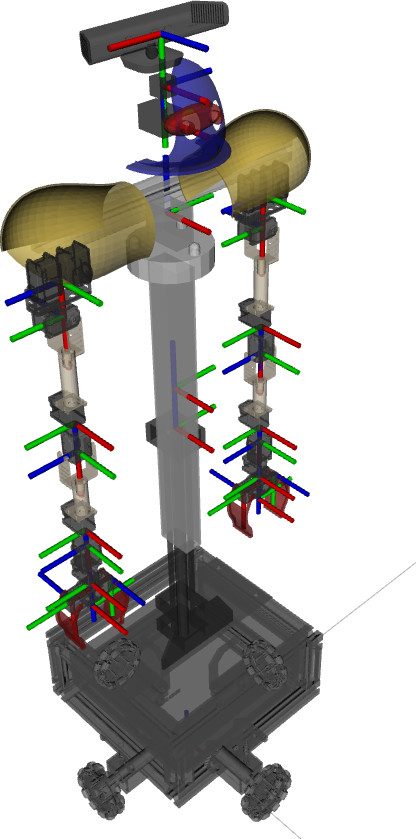
\includegraphics[scale=0.24]{manipulator/DH_manipulators1.png}
		\caption{URDF descripción del robot Justina.}
	\end{subfigure}%
	\begin{subfigure}[t]{.55\textwidth}
		\centering
		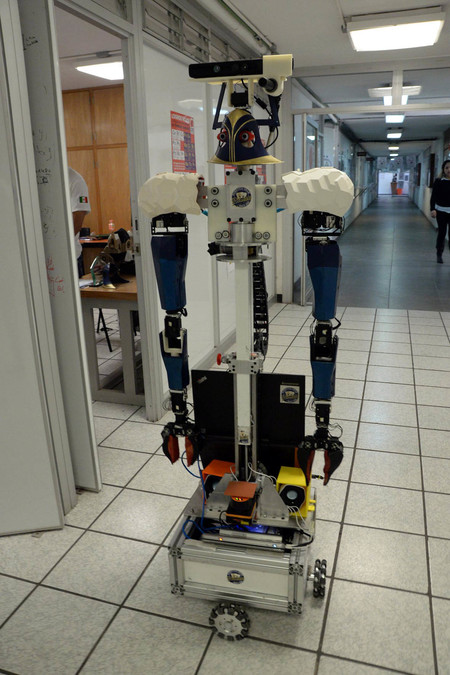
\includegraphics[scale=1.1]{manipulator/justina_real.jpg}
		\caption{Fotografía del robot Justina.}
	\end{subfigure}
	\caption{Imagen de Justina virtual y fotografia real.}
	\label{fig:desciption_arms1}
	\end{figure}




	En cuanto a la estructura de software, Justina se encuentra, actualmente, desarrollada en ROS; por tanto existen nodos encargados de la comunicación directa con el hardware. En el caso de este trabajo los nodos más relevantes a nivel de hardware son: el nodo encargado de la comunicación con los motores Dynamixel y el nodo encargado de operar al sensor Kinect. La comunicación con estos dos dispositivos de hardware se realiza mediante tópicos.\\

	El nodo encargado de operar los motores está publicando en todo momento la posición actual de cada uno de los servomotores; por otro lado está a la escucha permanente que llegue un mensaje con la información de una posición objetivo.\\

	El nodo del sensor kinect, se encarga de obtener los datos y publicar dos mensajes con informaciones similares. Uno de estos mensajes contiene la información del sensor kinect (imagen de color e información de profundidad) obtenida tal cual del hardware, el otro mensaje proviene de la transformación de la información de profundidad del sensor con respecto de la base del robot.\\

	Las relaciones mecánicas del robot se encuentran definidas mediante la nomenclatura correspondiente a un archivo URDF con el cual ROS crea un árbol de transformaciones dinámico. Con tal información podemos obtener las transformaciones entre diferentes sistemas de referencia dentro del robot o con respecto a algún sistema de referencia en particular.\\

	Como parte de este trabajo se programó un nodo en ROS en cual, con la información de las respectivas transformaciones y la información de profundidad obtenida del sensor kinect, se calcula la información del objeto y sus características de ubicación espacial, dimensiones y orientación. El nodo se realizó en el lenguaje de programación orientada a objetos C++, por su parte, se comunica a través de ROS por medio de la recepción de información mediante la llegada de tópicos; por otro lado responde en un servicio con la información de los objetos: ubicación espacial y orientaciones.\\

	

\newpage
\thispagestyle{empty}
\mbox{}

\addtocounter{page}{-1}